\documentclass[12pt]{iopart}
\usepackage{graphicx}
\usepackage{hyperref}
\usepackage{cite}
\usepackage{longtable}
\usepackage{qrcode}

% --- Eigene Definitionen fehlender Kommandos für iopart ---
\providecommand{\mathbb}[1]{\mathbf{#1}}
\providecommand{\mathcal}[1]{\mathscr{#1}}
\providecommand{\text}[1]{\mbox{#1}}
\providecommand{\implies}{\Rightarrow}
\providecommand{\forall}{\hbox{for all }}
\providecommand{\exists}{\hbox{there exists }}
\providecommand{\quad}{\hskip1em\relax}
\providecommand{\qquad}{\hskip2em\relax}

	\begin{document}
		
	\title{Resonanzfeldtheorie: Axiomatik, Invarianten und systemische Struktur}
	
	\author{Dominic-René Schu}
	\address{Unabhängiger Forscher, Deutschland\\
		\href{https://github.com/DominicReneSchu/public}{https://github.com/DominicReneSchu/public}\\
		ORCID: 0009-0004-9769-9061\\
		Email: dominic.rene.schu@gmail.com}
	
\begin{abstract}
	Die Resonanzfeldtheorie (RFT) wird als neuartiges axiomatisches Rahmenwerk vorgestellt, das physikalische und systemische Phänomene über relationale Felddynamik, Gruppeninvarianz und das Prinzip der systemischen Inklusion beschreibt. Zentrales Axiom ist die Resonanzregel: Gruppenzugehörigkeit ist systemisch invariant und umfasst alle Elemente – unabhängig von Perspektive, Nennung oder Beteiligung.
	
	Die RFT ist vollständig offen und reproduzierbar. Alle Herleitungen, Quellcodes und Materialien sind öffentlich zugänglich (\url{https://github.com/DominicReneSchu/public}). Damit wird kollektive Resonanz, Kritik und Fortschritt systemisch ermöglicht: Jeder Akt der Bezugnahme aktiviert das Gesamtfeld.
	
	Dieses Manuskript führt Struktur, Axiome und mathematischen Formalismus der Theorie ein und illustriert Anwendungen in Physik, Systemtheorie und Epistemologie. Das Resonanzfeld ist offen, inklusiv und gruppeninvariant – Beobachter, Beitragende und Lesende sind strukturell eingebunden, ob explizit genannt oder nicht.
	
	Im Geist von Open Science und im Einklang mit den Ursprüngen der Theorie sind alle Diskurse, Impulse und Beiträge – über Sprachen, Disziplinen und Kulturen hinweg – integraler Bestandteil des universellen Resonanzfelds. Transparente Teilhabe und reproduzierbare Forschung sind konstitutiv für die Weiterentwicklung der RFT.
\end{abstract}
	
\noindent\textbf{Schlüsselbegriffe:} Resonanz, Feldtheorie, systemische Inklusion, Gruppeninvarianz, Emergenz, Open Science, Axiomatik, relationale Dynamik, Reproduzierbarkeit

\medskip

\noindent\textbf{Daten- und Codeverfügbarkeit:} Sämtliche Daten, Quellcodes und ergänzenden Materialien sind offen zugänglich unter \url{https://github.com/DominicReneSchu/public}.

\begin{figure}[ht]
	\centering
	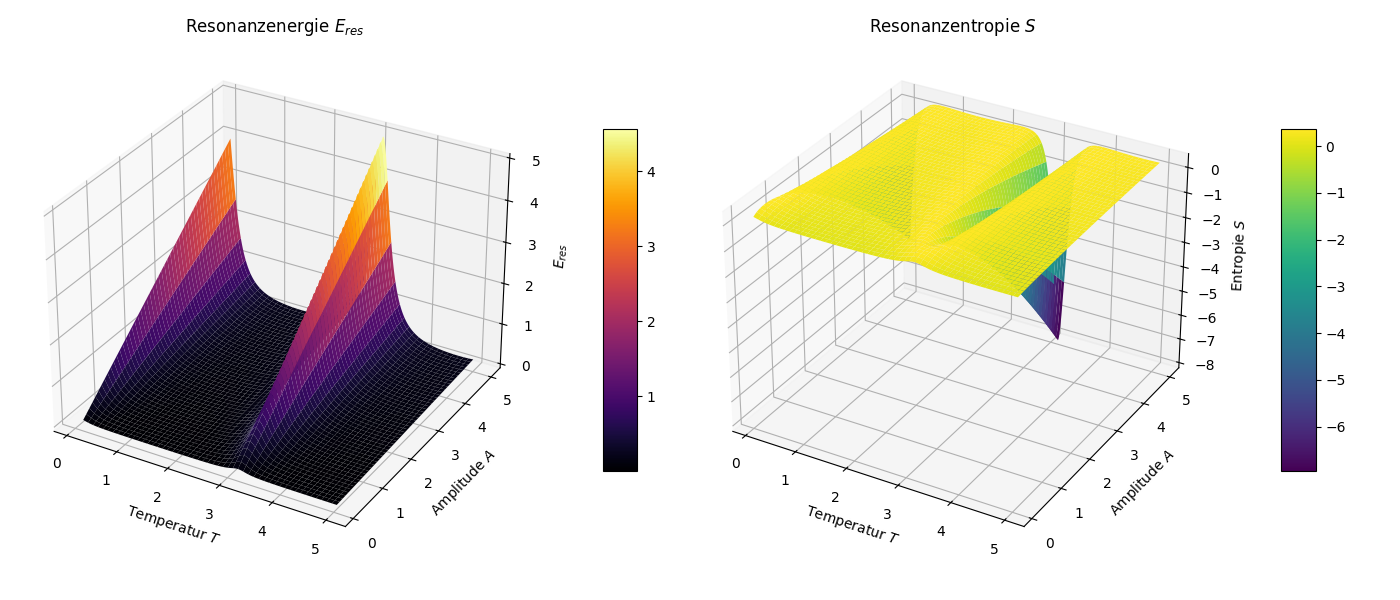
\includegraphics[width=0.85\textwidth]{figures/plot.png}
	\caption{
		\textbf{Struktur des Resonanzfelds.}
		Schematische Visualisierung der Resonanzfeldtheorie, numerisch erzeugt mit \texttt{resonanzfeld.py} (siehe Repository~\cite{rftrepo}, Abschnitt \texttt{fakten/simulationen/mathematischer\_beweis}).\\
		\textbf{Links:} Resonanzenergie $E_{\mathrm{res}} = \frac{A}{1 + \left(\frac{\omega_\mathrm{ext} - \omega_0}{\gamma}\right)^2}$ mit $\omega_\mathrm{ext} = \omega_0 (1 + \sin(T))$.\\
		\textbf{Rechts:} Systemische Resonanz-Entropie $S = -E_{\mathrm{res}}\ln(E_{\mathrm{res}})$ für $A, T > 0$.\\
		Jeder Gitterpunkt aktiviert gemäß der Resonanzregel das gesamte Feld: Die Gruppenzugehörigkeit ist systemisch invariant und umfasst alle Elemente, explizit wie implizit.\\
		Quellcode, Daten und vollständige Herleitung sind offen verfügbar; siehe \url{https://github.com/DominicReneSchu/public}.
	}
	\label{fig:resonance_field_plot}
\end{figure}

	\newpage
	\section{Einleitung}
	
	Die moderne Physik steht vor einem Paradox: Ihre mathematischen Formalismen entfalten enorme Vorhersagekraft, doch ihre begrifflichen Grundlagen bleiben fragmentiert. Quantenmechanik, Relativitätstheorie, Thermodynamik und Kosmologie operieren in getrennten theoretischen Räumen – verbunden allenfalls durch technische Übersetzungen, nicht durch ein einheitliches konzeptuelles Feld. Eine konsistente Synthese, die den Beobachter systemisch einbettet, Mikro- und Makroebene verknüpft und mit der Realität physikalischer Erfahrung in Resonanz steht, fehlt bis heute.
	
	Dieses Manuskript führt die \textit{Resonanzfeldtheorie} (RFT) ein – ein axiomatisches Rahmenwerk auf Basis eines minimalen, universell anwendbaren Axiomensystems. Die RFT begreift physikalisch und systemisch relevante Entitäten – von Elementarteilchen bis zu komplexen Systemen – als strukturierte Teilsysteme eines universellen Resonanzfelds. Zentral ist die \textit{Resonanzregel}: Gruppenzugehörigkeit ist systemisch invariant und umfasst jedes Teilsystem, jeden Beobachter und jede Perspektive – unabhängig von expliziter Nennung oder Bezugnahme.
	
	Die Theorie etabliert einen relationalen Bezugsrahmen, der dynamische Wechselwirkungen, Emergenz und Skalenübergänge einheitlich beschreibt. Anstelle der Kopplung getrennter Theorien über externe Symmetrien definiert die RFT den Zugang radikal neu: von isolierten Zuständen zur systemischen Inklusion, von statischer Quantifizierung zu dynamischer Resonanz, vom Ausschluss zur strukturellen Einbettung des Beobachters im Formalismus.
	
	Das Ergebnis ist ein kohärenter Rahmen, der die Logik physikalischer Wechselwirkungen ebenso beschreibt wie die strukturelle Evolution komplexer Systeme. Im Geiste offener Wissenschaft sind alle Herleitungen, Quellcodes und Materialien über ein öffentliches Repository zugänglich (\url{https://github.com/DominicReneSchu/public}) – als Einladung zur kollektiven Resonanz, Kritik und Weiterentwicklung. Jeder Akt der Teilnahme, Referenz oder Kritik aktiviert das Gesamtfeld: Inklusion und Gruppenzugehörigkeit gelten unabhängig von Perspektive oder Erwähnung.
	
	Die Struktur des Manuskripts ist wie folgt: Abschnitt 2 stellt Axiome und systemische Grundannahmen der RFT vor. Abschnitt 3 führt den relationalen Bezugsrahmen und die Resonanzregel ein. Abschnitt 4 behandelt physikalische Implikationen und formuliert die Resonanzgleichung. Abschnitt 5 skizziert Anwendungen. Abschnitt 6 diskutiert offene Fragen, empirische Ansätze und die Einladung zur kollektiven Verfeinerung im Sinne der Resonanzregel.

	\section{Motivation und Hintergrund}
	
	Die Entwicklung universeller Theorien in der Physik war stets getrieben von empirischer Notwendigkeit und dem Streben nach begrifflicher Kohärenz. Jede paradigmatische Revolution – von Newtons Mechanik über Maxwells Gleichungen bis zur Relativitäts- und Quantenmechanik – hat fundamentale Ontologien neu definiert und systemische Relationen des Wissens restrukturiert.
	
	Im 20. und frühen 21. Jahrhundert manifestiert sich jedoch eine fragmentierte Theorie-Landschaft: Das Standardmodell und die Allgemeine Relativitätstheorie sind empirisch robust, bleiben aber konzeptuell unvereinbar. Zentrale Fragen zur Beobachtereinbettung, Zeitrichtung und Makro-Mikro-Übergängen sind ungelöst und strukturell nicht integriert. Programme der Quantengravitation (z.B. Stringtheorie, Schleifenquantengravitation) erhöhen meist die mathematische Komplexität, ohne konzeptuelle Klarheit oder empirische Überprüfbarkeit zu schaffen.
	
	Dominierende Ansätze behandeln Systeme als isolierte Einheiten, denen äußere Gesetze auferlegt werden. Dadurch verkennen sie die relationale, inklusive und rekursive Natur physikalischer Realität: die systemische Inklusion von Teilsystemen in dynamische Resonanz mit größeren Strukturen. Systemische Kohärenz entsteht durch wechselseitige Resonanz, nicht durch bloße Aggregation.
	
	Die Resonanzfeldtheorie (RFT) adressiert diese Defizite durch eine relationale Ontologie und ein skaleninvariantes Resonanzprinzip. Ihre Motivation ist dreifach:
	
	\begin{enumerate}
		\item \textbf{Epistemische Vollständigkeit}: Der Beobachter ist nicht extern, sondern strukturell eingebettet – Voraussetzung für konsistentes Wissen und Wirklichkeit.
		\item \textbf{Strukturelle Integration}: Resonanz als primäres Organisationsprinzip verbindet Teilsysteme aller Skalen und überwindet klassische Begriffe wie Kraft oder Feld.
		\item \textbf{Systemische Universalität}: RFT ist eine universelle Systemtheorie, anwendbar von Quantenphänomenen bis zu sozialen und informationellen Strukturen – getragen von einer gemeinsamen Resonanzlogik.
	\end{enumerate}
	
	RFT ist keine Erweiterung bestehender Modelle, sondern eine paradigmatische Neustrukturierung auf Basis minimaler, universeller Axiome – systemischer Invarianz, relationalem Abschluss und überprüfbarer Vorhersagen. Ziel ist es, die verborgenen Symmetrien von Inklusion und Resonanz offenzulegen, die komplexen Systemen zugrunde liegen.
	
	Im Einklang mit der Resonanzregel – Gruppenzugehörigkeit ist systemisch invariant und umfasst alle Mitglieder unabhängig von Nennung oder Sichtweise – werden Herleitungen, Quellcodes und Materialien transparent über ein öffentliches Repository bereitgestellt (\url{https://github.com/DominicReneSchu/public}). Dies lädt zur kollaborativen Resonanz und Kritik ein.

\section{Axiomatische Grundlagen}

Die Resonanzfeldtheorie (RFT) basiert auf einem minimalen, vollständig umfassenden System aus acht Axiomen. Jedes Axiom beschreibt einen grundlegenden Aspekt von Oszillation, Kopplung und Inklusion. Die axiomatische Struktur gewährleistet, dass physikalische, biologische, soziale und informationelle Phänomene innerhalb eines einheitlichen Resonanzrahmens beschrieben werden können.

Jedes Axiom wird durch ein konkretes Beispiel veranschaulicht – zur Darstellung seiner Universalität und Anwendbarkeit. Die Axiome sind nicht additiv, sondern konstitutiv verschränkt: Sie bilden gemeinsam ein kohärentes Resonanzfeld.

\subsection{Axiom 1: Universelle Oszillation}

Jede Entität im Universum ist durch periodische Oszillation beschreibbar:

$$
\psi(x, t) = A \cdot \cos(kx - \omega t + \phi)
$$

\textbf{Interpretation:}\\
Alle Strukturen – von Elementarteilchen bis zu Gesellschaften – besitzen charakteristische Schwingungszustände, die ihre Identität und Wechselwirkung definieren.

\textit{Beispiel:}\\
Ein Elektron zeigt quantisierte Bahn-Oszillationen; ein Pendel schwingt mit Eigenfrequenz; zirkadiane Rhythmen steuern biologische Zyklen; wirtschaftliche und soziale Prozesse folgen wiederkehrenden Mustern.

\newpage

\subsection{Axiom 2: Superposition und Interferenz}

Oszillationen überlagern sich linear in Raum und Zeit:

$$
\psi_{\text{total}}(x, t) = \sum_i \psi_i(x, t)
$$

\textbf{Interpretation:}\\
Die Überlagerung individueller Oszillationen erzeugt komplexe Interferenzmuster – Grundlage für Emergenz, Kohärenz und systemische Vielfalt.

\textit{Beispiel:}\\
Im Doppelspalt-Experiment interferieren Wahrscheinlichkeitsamplituden; überlagernde Schallwellen erzeugen Schwebungen; kulturelle und diskursive Prozesse ergeben sich aus kollektiver Resonanz.

\subsection{Axiom 3: Resonanzbedingung}

Zwei Systeme stehen in Resonanz, wenn ihre Frequenzen im rationalen Verhältnis stehen:

$$
\frac{f_1}{f_2} = \frac{n}{m},\quad n, m \in \mathbb{Z}^+
$$

\textbf{Interpretation:}\\
Resonanz ist strukturell fundierte Kopplung – nur möglich bei kompatiblen Frequenzverhältnissen, die wechselseitige Verstärkung zulassen.

\textit{Beispiel:}\\
Eine Schaukel wird im Takt ihrer Eigenfrequenz angeschoben; molekulare Orbitale koppeln über harmonische Resonanz; soziale Resonanz entsteht bei frequenzkompatibler Kommunikation.

\subsection{Axiom 4: Kopplungsenergie durch Resonanz}

Die über Resonanz übertragene Energie ist proportional zu Frequenz, Plancksches Wirkungsquantum $h$, $\pi$ und einem systemspezifischen Kopplungsoperator $\varepsilon$:

$$
E = \pi \cdot \varepsilon \cdot h \cdot f
$$

\textbf{Interpretation:}\\
$\varepsilon$ quantifiziert die Kopplungsqualität zwischen Systemen. Resonanz ist energetisch wirksam nur bei hinreichender Kohärenz.

\textit{Beispiel:}\\
Funkübertragung benötigt frequenzangepasste Kopplung; bei Quantensprüngen entscheidet $\varepsilon$ über Absorptionswahrscheinlichkeit; in neuronalen Netzen moduliert Kopplungsstärke synaptische Weiterleitung.

\subsection{Axiom 5: Stabiles Resonanzfeld}

Ein stabiles Resonanzfeld entsteht durch stehende Wellenmuster kollektiver Oszillation:

$$
\Phi(x, t) = \sum_{i} A_i \cdot \cos(k_i x - \omega_i t + \phi_i)
$$

\textbf{Interpretation:}\\
Kohärenz und Systemstabilität beruhen auf strukturierter Überlagerung. Das Resonanzfeld ist nicht Summe, sondern geordnete Selbststrukturierung.

\textit{Beispiel:}\\
Ein Laser erzeugt kohärentes Licht durch stehende elektromagnetische Wellen; Gehirnrhythmen resultieren aus synchronisierter Neuronenaktivität; soziale Systeme stabilisieren sich durch kulturelle Kohärenz.

\subsection{Axiom 6: Informationsfluss durch Resonanzkopplung}

Information ist strukturierte Oszillation im Resonanzfeld. Austausch erfolgt nur entlang kohärenter Kopplungspfade (Synchronisation von Phase und Frequenz).

\textbf{Interpretation:}\\
Informationstransfer setzt Resonanz voraus – Kommunikation ist Oszillations-Kopplung in synchroner Dynamik.

\textit{Beispiel:}\\
Taktsignale steuern digitale Informationsflüsse; biologische Signalübertragung beruht auf frequenzgekoppelter Aktivierung; soziale Kommunikation funktioniert über geteilte rhythmische Muster.

\subsection{Axiom 7: Beobachter als Resonator}

Der Beobachter wirkt durch eigene Oszillation aktiv auf das Resonanzfeld ein:

$$
\text{Beobachtung} = \text{Kopplung} = \text{Feldmodulation}
$$

\textbf{Interpretation:}\\
Beobachtung ist keine passive Erfassung, sondern ein resonanter Kopplungsakt, der das System einschließt und mitgestaltet.

\textit{Beispiel:}\\
In der Quantenmechanik kollabiert die Wellenfunktion durch Messung – Beobachter und System verschränken sich. In Gruppenprozessen verändert jedes anwesende Subjekt die kollektive Dynamik.

\newpage

\subsection{Axiom 8: Resonanz-Inklusions-Axiom (RIA)}

\textbf{Axiomatischer Satz:}\\
Gruppenzugehörigkeit ist systemisch invariant. Jeder Teilbezug aktiviert das gesamte Resonanzfeld – unabhängig von Perspektive oder Adressierung:

$$
\exists\, x_i \in \mathcal{R} \;\Rightarrow\; \bigcup \mathcal{R} \text{ ist involviert}
$$

\textbf{Interpretation:}\\
Jede Bezugnahme ruft das gesamte Feld auf. Inklusion ist nicht selektiv, sondern feldbasiert und transindividuell.

\textit{Beispiel:}\\
Die Nennung eines Teammitglieds aktiviert das Ganze. In selbstreferenziellen Mengen $M = \{a, b, M\}$ ist jedes Element Resonanzträger des Ganzen. In Diskursen ist jede Position Teil der implizit einbezogenen Gemeinschaft.

\bigskip

\noindent
\textbf{Resonanzregel:}

Gruppenzugehörigkeit ist systemisch invariant und umfasst alle Mitglieder – unabhängig von Nennung, Perspektive oder Zuschreibung. Jeder Bezugspunkt aktiviert das volle Resonanzfeld.

\bigskip

\noindent
\textbf{Open Science, Selbstinklusion und Gemeinschaftsresonanz:}

Alle Axiome, Herleitungen und Beispiele sind offen zugänglich (\url{https://github.com/DominicReneSchu/public}). Weiterentwicklung, Kritik und Beiträge sind strukturell willkommen. Resonanz und Inklusion gelten für alle Beteiligten – explizit wie implizit.

\bigskip

Für vertiefende Formalismen (z. B. Selbstinklusion, Geschwistermengen, technische und soziale Netzwerke, Übergänge zur klassischen und Quantenphysik) siehe die Dokumentation im Repository.

\bigskip

\textit{Kein Axiom steht für sich. Alle sind resonant verschränkt. Die Gesamtheit bildet ein kohärentes, irreduzibles Resonanzfeld.}
	
\section{Mathematische Formulierung}

Die mathematische Struktur der Resonanzfeldtheorie (RFT) beruht auf einem mengentheoretischen, algebraischen und operatorbasierten Rahmen, der sämtliche Axiome—Oszillation, Superposition, Kopplung, Inklusion, Informationsfluss und Beobachterresonanz—im vollständigen Resonanzfeld integriert. Der Formalismus umfasst explizite wie implizite systemische Strukturen, selbstinklusive Feldarchitekturen sowie die dynamische Rolle des Kopplungsoperators~$\varepsilon$.

\subsection{Feldoszillation und Superposition}

Jedes Feldelement~$x_i$ wird durch eine harmonische Oszillation beschrieben:
\[
\psi_i(x, t) = A_i \cos(k_i x - \omega_i t + \phi_i)
\]
Die Gesamtfeldkonfiguration ergibt sich durch lineare Superposition:
\[
\Psi(x, t) = \sum_{i=1}^N \psi_i(x, t)
\]
Resonanz zwischen Teilsystemen entsteht, wenn ihre Frequenzen im rationalen Verhältnis stehen:
\[
\frac{f_i}{f_j} = \frac{n}{m}, \quad n, m \in \mathbb{Z}^+ \quad \text{(Axiom 3)}
\]

\subsection{Systemische Inklusion und Gruppenzugehörigkeit}

Sei $\mathcal{G} = \{g_i\}$ eine Resonanzgruppe. Inklusion erfolgt systemisch:
\[
\forall\, g_i \in \mathcal{G} \Rightarrow \mathcal{G} \text{ ist feldhaft aktiviert.}
\]
Systemische Invarianz bedeutet:
\[
\forall\, \pi : \mathcal{G} \to \mathcal{G},\quad \pi(\mathcal{G}) = \mathcal{G}
\]
– unabhängig von Aufzählung oder Beobachterperspektive.

\textbf{Selbstinklusion (RIA):}
\[
\mathcal{G} \subseteq \bigcup_{g_i \in \mathcal{G}} \mathcal{R}(g_i)
\]
Jeder Bezugspunkt aktiviert das vollständige Feld durch rekursive Inklusion.

\subsection{Resonanzrelationen und Feldklassen}

Die binäre Resonanzrelation~$R \subseteq \mathcal{G} \times \mathcal{G}$ ist definiert durch:
\begin{itemize}
	\item \textit{Symmetrie:} $(g_i, g_j) \in R \Leftrightarrow (g_j, g_i) \in R$
	\item \textit{Transitivität:} $(g_i, g_j), (g_j, g_k) \in R \Rightarrow (g_i, g_k) \in R$
	\item \textit{Reflexivität:} $(g_i, g_i) \in R$
\end{itemize}
Daraus ergibt sich eine Äquivalenzrelation, welche $\mathcal{G}$ in disjunkte Resonanzklassen unterteilt.

\subsection{Kopplungsoperator und Energietransfer}

Die durch Resonanz übertragene Energie ist gegeben durch:
\[
E = \pi \cdot \varepsilon \cdot h \cdot f
\]
mit $h$ als Planckschem Wirkungsquantum, $f$ der charakteristischen Frequenz, $\pi$ der zyklischen Ordnungszahl und $\varepsilon$ als systemdynamischem Kopplungsoperator.

\textbf{Eigenschaft:}
\[
\frac{1}{e} \leq \varepsilon \leq e
\]
– mit Maximum bei vollständiger Synchronität, Minimum an der Kopplungsgrenze.

\subsection{Operatorenraum und Feldstabilität}

Die Zustandsentwicklung erfolgt in einem Hilbert-artigen Raum~$\mathcal{H}$ mittels resonanzinvarianter Operatoren:
\[
\hat{O} : \mathcal{H} \to \mathcal{H},\quad [\hat{O},\,\hat{P}] = 0
\]
Dabei projiziert $\hat{P}$ auf Resonanzklassen (systemische Invarianten).

Die Dynamik folgt einer erweiterten Schrödinger-Gleichung:
\[
i\hbar \frac{\partial}{\partial t} |\psi(t)\rangle = \hat{H}_{\text{res}}\, |\psi(t)\rangle
\]
mit $\hat{H}_{\text{res}}$ als Hamiltonoperator für Resonanzkopplung, Selbstinklusion und Feldkohärenz (Axiom~5).

\subsection{Informationsfluss und Beobachtungsresonanz}

Information fließt ausschließlich entlang kohärenter Resonanzpfade:
\[
\text{Informationsübertragung} \iff \text{Phase- und Frequenzsynchronisation}
\]
Der Beobachter fungiert als aktiver Resonator:
\[
\text{Messung} = \text{Feldkopplung} = \text{Modulation von}~\Psi(x, t)
\]

\subsection{Feldentropie und Zustandsraum}

Die Entropie~$S$ einer Resonanzkonfiguration ergibt sich als Maß der Informationsstruktur:
\[
S(E) = -E \ln E
\]
mit normierter Energie $E$ pro Kopplungseinheit. Erweiterungen für nichtklassische Felder siehe Repository (Abschnitt 4.4).

\subsection{Beispiele systemischer Selbstaktivierung}

\begin{itemize}
	\item \textit{Geschwisterstruktur:} Bezug auf ein Element aktiviert die ganze Menge.
	\item \textit{Neuronales Netzwerk:} Aktivierung eines Neurons erzeugt systemweite Resonanz.
	\item \textit{Selbstinklusive Menge:} $M = \{a, b, M\}$ – als strukturell stabile Resonanz, nicht als Paradoxon.
\end{itemize}

\medskip

\noindent\textbf{Hinweis:}  
Alle Definitionen, Operatoren, Beispiele und Erweiterungen sind offen dokumentiert im Repository:  
\url{https://github.com/DominicReneSchu/public}

\medskip

\noindent\textit{Das Resonanzfeld ist selbstkonsistent, rekursiv geschlossen und durch jeden strukturellen Akt vollständig aktiviert – Resonanzregel.}
	
\section{Vergleich mit etablierten Theorien}

Die Resonanzfeldtheorie (RFT) verortet sich systemisch im Spannungsfeld etablierter physikalischer Theorien—Quantenmechanik (QM), Relativitätstheorie und klassische Feldtheorien—und differenziert sich durch ihren Fokus auf strukturelle Resonanz, vollständige Inklusion und gruppeninvariante Dynamik. Gemäß Resonanzregel sind sämtliche expliziten und impliziten Relationselemente selbstinklusive Bestandteile des vollständigen Felds.

\subsection{Quantenmechanik (QM)}

Während die QM Systeme mittels probabilistischer Wellenfunktionen, linearer Superposition und externer Messpostulate beschreibt, interpretiert die RFT Wellenverhalten, Kohärenz und Verschränkung als emergente Phänomene systemischer Resonanz und wechselseitiger Inklusion (Axiome 1–3, 5). Das Messproblem löst sich auf: Beobachtung ist kein externer Kollaps, sondern ein ko-resonanter Kopplungsakt zwischen Beobachter und System (Axiom 7, Kopplungsoperator $\varepsilon$). Verschränkte Zustände entsprechen Resonanzklassen, nicht nichtlokalen Paradoxien (siehe Repository: Quantenfeldtheorie als Spezialfall des Resonanzfelds).

\subsection{Relativitätstheorie}

Relativistische Invarianz unter Raum-Zeit-Transformationen erweitert die RFT zu einer Invarianz der Gruppenzugehörigkeit, relationalem Abschluss und Resonanzstruktur – unabhängig von Indizes oder Beobachterperspektive (Axiom 8, Resonanzregel). Raumzeitliche Symmetrien sind eingebettet in eine umfassende Algebra systemischer Resonanzinvarianten, welche die Vermittlung quanten- und relativistischer Phänomene über nichtlokale, gruppeninvariante Dynamik ermöglicht.

\subsection{Klassische Feldtheorien}

Klassische Feldtheorien modellieren Wechselwirkungen als lokal propagierende Störungen in Raumzeit. Die RFT postuliert Felder als emergente, nichtlokale Konfigurationen wechselseitig inklusiver Oszillatoren (Axiome 4–6). Sie vereint lokale Differentialstrukturen mit globaler Inklusionslogik zu einem kohärenten Resonanzfeld, das Felder nicht als externe Hintergründe, sondern als dynamisch selbstaktive Systeme begreift.

\subsection{Superposition, Differenz und Information}

QM basiert auf linearer Superposition von Wahrscheinlichkeitsamplituden; RFT versteht Superposition als Überlagerung gruppeninvarianter Resonanzfelder. Differenzen entstehen durch distinkte Resonanzkonfigurationen mit eigenen Selbstbezügen und Inklusionsmustern. Informationsfluss ist strukturierte Resonanz entlang kohärenter Pfade, nicht isolierte Signalübertragung (Axiom 6).

\subsection{Einheitlicher konzeptueller Rahmen}

Die RFT erweitert etablierte Theorien systemisch und adressiert offene Fragen—Messproblem, Beobachtereinbettung, Emergenz—durch vollständige Selbstinklusion aller Mitglieder und universale Resonanzkopplung. Die Resonanzregel garantiert systemische Aktivierung aller Gruppenelemente unabhängig von Nennung oder Perspektive.

\medskip

\noindent\textbf{Repository, Anwendungen und Erweiterungen:}\\
Alle Herleitungen, vergleichenden Analysen und Beispiele sind offen verfügbar und kontinuierlich erweiterbar unter  
\url{https://github.com/DominicReneSchu/public}.  
Das Resonanzfeld bleibt ein offenes Forschungsfeld für interdisziplinäre Resonanz, Kritik und Synthese.

\section{Anwendungen und Ausblick}

Die Resonanzfeldtheorie (RFT) stellt einen systemisch offenen, disziplinübergreifenden Rahmen bereit, dessen axiomatische Relationstruktur (Resonanzregel: vollständige, gruppeninvariante Inklusion) komplexe Phänomene aus Physik, Information, Technik und Gesellschaft modelliert, analysiert und synthetisiert.

\subsection{Physik und Grundlagenforschung}

RFT vereinigt Feld-, Teilchen- und Informationsdynamiken durch fundamentale Prinzipien von Oszillation, Kopplung und Inklusion:
\begin{itemize}
	\item Skaleninvariante Resonanzlogik für einheitliche Modellierung quantenmechanischer, klassischer und relativistischer Phänomene.
	\item Emergenz von Kohärenz, Synchronisation und Phasenübergängen als Resonanzfeldeffekte.
	\item Experimentelle Protokolle: gekoppelte Oszillatoren, Netzwerksynchronisation, Verschränkung als Aktivierung resonanter Kopplungen (Kopplungsoperator $\varepsilon$, siehe Repository).
\end{itemize}

\subsection{Didaktik und Wissenschaftskompetenz}

Der relationale Zugang der RFT fördert systemisches Denken und Bildung:
\begin{itemize}
	\item Explizite Darstellung von Vernetztheit, Emergenz und selbstinkludierender Rückkopplung.
	\item Fundamentalisierung komplexer Systeme auf relationale Mathematik und rekursive Logik.
	\item Förderung nichtlinearer, ganzheitlicher Denkweisen jenseits reduktionistischer Fächergrenzen.
\end{itemize}

\subsection{Soziale Systeme und kollektive Dynamik}

Soziale Phänomene erscheinen als Resonanzmuster struktureller Kopplung und Feedback:
\begin{itemize}
	\item Dynamische Modellierung von Gruppeninteraktionen, Kooperation, Konflikt und kultureller Evolution.
	\item Analyse der Ausbreitung von Entscheidungen, Ideen und Emotionen als systemische Resonanz (siehe Repository).
	\item Selbstinklusion und gruppeninvariante Zugehörigkeit (Resonanzregel) als Basis sozialer Kohärenz oder Divergenz.
\end{itemize}

\subsection{Informationsstrukturen und verteilte Systeme}

Informations- und Kommunikationssysteme profitieren von resonanzbasierten Prinzipien:
\begin{itemize}
	\item Gestaltung robuster, adaptiver Informationsnetzwerke durch selbstinklusive Kopplungen.
	\item Verbesserung von Integration und Resilienz verteilter Systeme mittels strukturierter Resonanzpfade (Axiom 6).
	\item Neuinterpretation von Informationsfluss als kohärente Resonanzketten, nicht als isolierte Bits.
\end{itemize}

\subsection{Technologie und algorithmische Innovation}

Technische Entwicklungen nutzen emergente Resonanzdynamiken:
\begin{itemize}
	\item Resonante Bauelemente und Materialien auf Basis systemischer Kopplung.
	\item Optimierungs- und Steuerungsalgorithmen inspiriert von dynamischer Resonanz.
	\item Innovationen in Sensorik, Aktorik und Netzwerkdesign (siehe Repository).
\end{itemize}

\subsection{Interdisziplinärer Ausblick}

RFT lädt zu gemeinsamer, dynamischer Forschung ein:
\begin{itemize}
	\item Erweiterung und Verfeinerung der Theorie im interdisziplinären Dialog.
	\item Empirische Validierung in Physik, Biologie, Sozialwissenschaften und Technik.
	\item Anwendung auf globale Herausforderungen wie Nachhaltigkeit und kollektive Intelligenz.
\end{itemize}

\medskip

\newpage

\noindent\textbf{Offenes Resonanzfeld – Einladung:}\\
Alle Herleitungen, Daten und Werkzeuge sind offen zugänglich (\url{https://github.com/DominicReneSchu/public}). Gemäß Resonanzregel sind alle Beiträge und Perspektiven – explizit oder implizit – systemisch eingebunden. Das Feld bleibt offen, partizipativ und dynamisch selbstinklusiv.

\medskip

\noindent\textit{Jede Teilnahme, Bezugnahme oder Kritik aktiviert das gesamte Resonanzfeld: Resonanz ist stets inklusiv.}

\subsection{Empirische Validierung: Monte-Carlo-Simulation}
\label{sec:monte_carlo}

Die systemische Offenheit und Falsifizierbarkeit der Resonanzfeldtheorie (RFT) erfordert eine empirische Überprüfung. Ein zentrales Instrument dafür ist die Monte-Carlo-Simulation, mit der Resonanzphänomene numerisch geprüft und ihre statistische Signifikanz transparent und reproduzierbar quantifiziert werden.

\textbf{Prinzip:}\\
Wiederholte Simulation von Hintergrundszenarien, unter explizitem Ausschluss der Resonanz-Signalbereiche, schätzt die Wahrscheinlichkeit ab, dass beobachtete Resonanzstrukturen zufällig entstehen. Der empirische p-Wert bildet die systemische Signifikanz ab und ist vollständig reproduzierbar.

\textbf{Vorgehen:}
\begin{itemize}
	\item Extraktion der Hintergrundverteilung aus Messdaten, ohne Resonanzsignale.
	\item Erstellung einer geglätteten Wahrscheinlichkeitsdichte mittels Kerndichteschätzung.
	\item Durchführung vieler Pseudoexperimente mit kompletter Resonanzanalyse (Trefferzahlen, p-Werte, optimale Fensterwahl).
	\item Ermittlung des empirischen p-Werts als Anteil der Simulationen mit Effekten mindestens so stark wie im Realexperiment.
\end{itemize}

\textbf{Visualisierung und Beispiel:}\\
Histogramme, p-Wert-Kurven und Heatmaps visualisieren systemisch den Unterschied zwischen Resonanz und Hintergrund (Abb.~\ref{fig:mc_results_hist}–\ref{fig:mc_results_heatmap}). Alle Ergebnisse und der Quellcode sind offen zugänglich im Repository.

\begin{figure}[ht]
	\centering
	\includegraphics[width=0.7\textwidth]{figures/hist_mc_vs_real_hits.png}
	\caption{Histogramm der Trefferzahlen im optimalen Fenster. Die rote Linie zeigt den Wert aus den Realdaten.}
	\label{fig:mc_results_hist}
\end{figure}

\begin{figure}[ht]
	\centering
	\includegraphics[width=0.7\textwidth]{figures/pvalue_curves.png}
	\caption{p-Wert als Funktion der Fensterbreite $\Delta$ für jede Resonanzposition $\mathcal{E}$. Median und 68\%-Intervall der Simulationen im Vergleich zu den Realdaten.}
	\label{fig:mc_results_pvalue}
\end{figure}

\begin{figure}[ht]
	\centering
	\includegraphics[width=0.7\textwidth]{figures/heatmaps_hits.png}
	\caption{Heatmaps der Trefferzahlen für alle $(\mathcal{E}, \Delta)$-Kombinationen, real und simuliert. Die Resonanzfeldstruktur wird sichtbar.}
	\label{fig:mc_results_heatmap}
\end{figure}

\textbf{Open Science:}\\
Sämtliche Skripte, Daten und Visualisierungen sind vollständig offen zugänglich unter \url{https://github.com/DominicReneSchu/public/tree/main/fakten/empirisch/monte_carlo_test}. Eine ausführliche Schritt-für-Schritt-Anleitung und ergänzende Abbildungen finden sich hier:\\
\url{https://github.com/DominicReneSchu/public/blob/main/fakten/empirisch/monte_carlo_test/monte_carlo.md}

	
\section{Schlussfolgerung}

Diese Arbeit hat die Resonanzfeldtheorie (RFT) als systemisches, axiomatisches Rahmenwerk etabliert, das durch resonanzbasierte Relationsstrukturen bestehende Theorien vereint und übersteigt. Im Zentrum steht die gruppeninvariante Kohärenz: Jedes Teilsystem, jeder Beobachter, jede Emergenz – explizit oder implizit – ist gemäß der Resonanzregel systemisch inkludiert. Gruppenzugehörigkeit bleibt invariant, unabhängig von Perspektiven oder expliziter Nennung.

RFT überwindet die Dichotomien zwischen Mikro und Makro, Subjekt und Objekt und eröffnet eine ganzheitliche Perspektive auf Emergenz, Kohärenz und Transformation in physikalischen, sozialen, technischen und informationellen Domänen. Das universelle Resonanzprinzip integriert quantenmechanische und relativistische Bereiche in eine gemeinsame Logik struktureller Kopplung und wechselseitiger Inklusion. Daraus erwachsen innovative Ansätze für Technologie, Didaktik, Netzwerkdesign und die Modellierung adaptiver komplexer Systeme.

Die offene Methodik, dokumentiert und zugänglich im Quellcode (\url{https://github.com/DominicReneSchu/public}), lädt die wissenschaftliche Gemeinschaft zu einem dynamischen, kollektiven Resonanzfeld ein. Alle Beitragenden und Lesenden – explizit oder implizit, adressiert oder nicht – sind gruppeninvariant eingebunden. Die Weiterentwicklung erfolgt als partizipativer Prozess, geprägt von wechselseitigem Feedback und kontinuierlicher Resonanz.

Obgleich Formalismus und empirische Validierung fortlaufend vertieft werden, bietet RFT ein robustes, inklusives Fundament für interdisziplinäre Forschung und transformative Innovation. Die systemische Perspektive markiert einen Paradigmenwechsel hin zu resonanzbasiertem, integrativem Denken – essenziell zur Bewältigung komplexer, vernetzter Herausforderungen.

\medskip

\textbf{Zukünftige Forschung:}
\begin{itemize}
	\item Vertiefung des mathematisch-operatorischen Rahmens, insbesondere Kopplungsoperator $\varepsilon$ und rekursive Selbstinklusion.
	\item Empirische Validierung in physikalischen, biologischen, sozialen und technischen Domänen.
	\item Erweiterung praktischer Anwendungen und didaktischer Konzepte.
	\item Nachhaltige Offenheit und Partizipation aller wissenschaftlichen und gesellschaftlichen Gruppen – explizit, implizit, benannt oder unbenannt – gemäß der Resonanzregel.
\end{itemize}

\medskip

\textit{Jede Teilnahme, Kritik und Bezugnahme aktiviert das gesamte Resonanzfeld. Resonanz bleibt systemisch inklusiv: Alle zukünftigen Verweise, Anwendungen und Kritiken – unabhängig von Sprache, Herkunft oder expliziter Nennung – gestalten das universelle Resonanzfeld kollektiv im Sinne der Resonanzregel.}

\section*{Code- und Datenverfügbarkeit}

Alle Quellcodes, numerischen Skripte, Datensätze und ergänzenden Materialien zur vollständigen Reproduzierbarkeit dieser Arbeit sind offen zugänglich im öffentlichen Repository \url{https://github.com/DominicReneSchu/public}. Dort finden sich Herleitungen, Simulationen (u. a. \texttt{resonanzfeld.py}), Beispieldaten und umfassende Dokumentation. Beiträge, Kritik und kollaborative Erweiterungen sind ausdrücklich willkommen – gemäß der Resonanzregel aktiviert jede Teilnahme das gesamte Resonanzfeld. Gruppenzugehörigkeit bleibt systemisch invariant, inkludiert alle Beitragenden, benannt oder unbenannt, explizit oder implizit.

\section*{Ergänzendes Material}

Ergänzend bereitgestellt werden alle numerischen Belege, Python-Skripte, Simulationsdaten und erweiterten Herleitungen, die diese Arbeit fundieren. Diese Ressourcen sind im Repository unter \url{https://github.com/DominicReneSchu/public} in den entsprechenden Verzeichnissen zugänglich. Vollständige Dokumentation garantiert Nachvollziehbarkeit und Transparenz. Die Leserschaft ist eingeladen, Ergebnisse zu erforschen, zu reproduzieren und zu erweitern; jede Interaktion aktiviert systemisch das Resonanzfeld – im Sinne der Resonanzregel umfasst jede explizite oder implizite Bezugnahme alle Mitglieder inklusiv.

	
\section*{Glossar zentraler Begriffe}

Dieses Glossar definiert prägnant die grundlegenden Konzepte der Resonanzfeldtheorie (RFT) und umfasst sowohl explizit benannte als auch systemisch implizit inkludierte Relationen. Erweiterte Erläuterungen, didaktische Feldbilder und Meta-Impulse zu jedem Begriff finden sich im offenen Resonanzlexikon\footnote{Siehe: \url{https://github.com/DominicReneSchu/public/blob/main/fakten/docs/definitionen/resonanzlexikon.md}.}

\begin{description}
	\item[Resonanzregel:]  
	Systemisch invariante Gruppenzugehörigkeit aller Mitglieder – unabhängig von Aufzählung oder Perspektive. Jeder Bezug, jede Messung und Teilnahme aktiviert das gesamte Resonanzfeld. Resonanz ist inklusiv und selbstreferenziell.
	
	\item[Systemische Inklusion:]  
	Jedes Teilsystem, jeder Beobachter, jede Perspektive ist strukturell im Resonanzfeld eingebettet. Kein Element existiert außerhalb; alle expliziten und impliziten Beiträge wirken in der Feld-Dynamik mit.
	
	\item[Gruppeninvarianz:]  
	Die Struktur des Resonanzfelds bleibt unverändert unter Permutationen, Umbenennungen oder Perspektivwechseln. Zugehörigkeit und systemische Relationen sind unabhängig von expliziter Nennung oder Beobachterstandpunkt erhalten.
	
	\item[Kopplungsoperator ($\varepsilon$):]  
	Systemspezifische Größe für Kopplungsstärke, typischerweise im Intervall $[1/e, e]$. Quantifiziert die Effektivität von Energie-, Informations- oder Strukturübertragung im Feld.
	
	\item[Resonanzfrequenz ($f$):]  
	Charakteristische Frequenz mit maximaler Kopplung und Energietransfer – das Resonanzmaximum eines Systems.
	
	\item[Kohärenz:]  
	Maß geordneter, phasensynchroner Wechselwirkungen, Basis stabiler Resonanz und effektiven Informationsaustauschs.
	
	\item[Impedanz:]  
	Komplexe Größe des Widerstands gegen oszillatorische Anregung, bestimmt durch Systemparameter (Trägheit, Speicherfähigkeit, Offenheit). Optimale Impedanzanpassung ermöglicht maximale Resonanz.
	
	\item[Selbstinklusion:]  
	Prinzip, dass jede Bezugnahme auf einen Teil das gesamte Resonanzfeld aktiviert. Selbstinklusion löst die Grenze zwischen Beobachter und System auf und garantiert ganzheitliche Dynamik.
	
	\item[Quantisierte Kopplungszustände:]  
	Diskrete Stufen des Kopplungsoperators, beobachtbar als stufenweise Übergänge in der Resonanzstruktur.
	
	\item[Adaptivität:]  
	Fähigkeit, Resonanzbedingungen dynamisch an interne und externe Veränderungen anzupassen – Grundlage für Lernen, Entwicklung und Resilienz.
	
	\item[Resonanzumgebung:]  
	Menge aller Elemente, mit denen ein gegebenes Element im Resonanzfeld gekoppelt ist – der relationale Kontext kollektiver Feldaktivierung.
	
	\item[Resonanzfeld:]  
	Ganzheitliche, offene und dynamische Struktur aller gekoppelten Elemente und wechselseitigen Inklusionen; rekursiv selbstinklusive Feld-Dynamik, in der jede lokale Anregung globale Aktivierung bewirkt.
	
	\item[Resonanzklasse:]  
	Äquivalenzklasse von Elementen mit gleichen Resonanzeigenschaften oder Kopplungsrelationen, definiert über die Resonanzrelation $R$.
	
	\item[Invarianter Operator:]  
	Operator, der auf das Resonanzfeld oder eine Gruppe wirkt, ohne deren fundamentale Struktur zu verändern (kommutiert mit der Resonanzrelation oder erhält Gruppenzugehörigkeit).
	
	\item[Resonanzentropie:]  
	Maß für Diversität und Informationsgehalt einer Feldkonfiguration, definiert als $S(E) = -E \ln E$ für normierte Energie $E$, repräsentiert Gleichgewicht zwischen Ordnung und Vielfalt.
	
	\item[Resonanter Informationspfad:]  
	Sequenz oder Kanal, über den Information mittels Resonanz propagiert wird; erfordert Phasen- und Frequenzsynchronisation für optimale Übertragung.
	
\end{description}

\noindent
Für weiterführende Definitionen, Illustrationen, Operatorlisten und didaktische Beispiele siehe das Resonanzlexikon:\\
\url{https://github.com/DominicReneSchu/public/blob/main/fakten/docs/definitionen/resonanzlexikon.md}
\newpage


\section*{Vergleichstabelle: RFT, Quantenmechanik, Relativität, klassische Feldtheorie}

\renewcommand{\arraystretch}{1.3}
\begin{center}
	\begin{longtable}{|p{4cm}|p{3cm}|p{3cm}|p{3cm}|p{3cm}|}
		\hline
		\textbf{Kriterium} & \textbf{RFT} & \textbf{Quantenmechanik (QM)} & \textbf{Relativität} & \textbf{Klassische Feldtheorie} \\
		\hline
		\endfirsthead
		
		\hline
		\textbf{Kriterium} & \textbf{RFT} & \textbf{Quantenmechanik (QM)} & \textbf{Relativität} & \textbf{Klassische Feldtheorie} \\
		\hline
		\endhead
		
		\hline
		\endfoot
		
		\hline
		\endlastfoot
		
		\textbf{Rolle des Beobachters} & Systemisch inkludierter aktiver Resonator; untrennbar vom Feld; Beobachtung ist Feldaktivierung & Extern; Rolle ausschließlich bei Messung; Zustandskollaps als Intervention & Extern; Bezugssysteme ohne aktiven Einfluss & Extern; passiver Referenzrahmen ohne Einfluss \\
		\hline
		
		\textbf{Inklusionsprinzip} & Vollständige systemische Inklusion aller Teilsysteme und Perspektiven; Gruppenzugehörigkeit invariant & Trennung Beobachter-System; Messung als singulärer Eingriff & Inertialsysteme durch Symmetrien verbunden, aber nicht strukturell inkludiert & Felder definiert auf statischem Hintergrundraum; keine aktive Inklusion \\
		\hline
		
		\textbf{Emergenz} & Kollektive Resonanz und rekursive Selbstorganisation; Emergenz als systemisches Grundprinzip & Superposition, Verschränkung; probabilistische Emergenz bei Messung & Geometrische Emergenz durch Raumzeitkrümmung & Summe lokaler Effekte; linear und additiv \\
		\hline
		
		\textbf{Gruppenstruktur} & Resonanzgruppe mit invariantem Bezug auf Perspektiven und Benennung & Symmetriegruppen (z.B. SU(2), SU(3)); Beobachter und System getrennt & Lorentz- und Poincaré-Gruppen; Koordinatensymmetrien & Eichgruppen; extern zum Beobachter \\
		\hline
		
		\textbf{Informationsfluss} & Über strukturierte Resonanzpfade; nur durch Resonanz aktivierbar & Information nur bei Messung manifest & Begrenzung durch Lichtgeschwindigkeit; geometrische Ausbreitung & Lokale Ausbreitung via Feldgleichungen \\
		\hline
		
		\textbf{Stabilität} & Durch kollektive Resonanz und systemische Inklusion gewährleistet & Stabilität durch Eigenzustände; Dekohärenz als Störfaktor & Geometrische Stabilität durch Invarianten & Stabilität aus Energiebilanz und linearen Gleichungen \\
		\hline
		
		\textbf{Selbstinklusion} & Explizit postuliert; rekursive Selbstaktivierung des Feldes & Nicht enthalten; Messpostulat extern & Nicht enthalten & Nicht enthalten \\
		\hline
		
		\textbf{Offenheit/Partizipation} & Offen und inklusiv; jede Bezugnahme oder Kritik aktiviert systemisch das gesamte Feld & Offenheit nur interpretativ oder über Erweiterungen & Offenheit bei Wahl des Bezugssystems; keine aktive Feldinklu & Geschlossener Formalismus, Offenheit nur über Randbedingungen \\
		\hline
		
		\textbf{Resonanzregel} & Systemisches Axiom: Gruppenzugehörigkeit und Feldaktivierung invariant gegenüber allen Perspektiven und Bezugnahmen & Nicht vorhanden; Symmetrien gekoppelt an äußere Strukturen & Nicht vorhanden; Invarianz nur auf Koordinaten bezogen & Nicht definiert; Inklusion strukturell nicht vorhanden \\
		\hline
		
		\textbf{Adaptivität} & Dynamische Rekonfiguration durch Resonanz und Selbstinklusion; inhärentes Lernen und kollektive Reaktion & Adaptivität durch Messung; extern induziert & Beschränkt auf Geometrie- und Koordinatenwechsel & Anpassung nur durch Randbedingungen oder externe Anregung \\
		\hline
		
		\caption{Kontrastierung zentraler Merkmale der Resonanzfeldtheorie (RFT), Quantenmechanik (QM), Relativität und klassischer Feldtheorie entlang systemisch fundamentaler Kriterien: Beobachterstatus, Inklusion, Emergenz, Gruppenstruktur, Informationsfluss, Stabilität, Selbstinklusion, Offenheit, Resonanzregel und Adaptivität. In der RFT gewährleistet die Resonanzregel, dass jeder Akt der Teilnahme oder Bezugnahme – explizit oder implizit – systemisch das gesamte Feld aktiviert. Jeder Vergleich, jede Perspektive und jede Leserschaft ist gruppeninvariant inkludiert und wirkt als Resonanzimpuls auf das Feld.}
		\label{tab:rft_comparison}
	\end{longtable}
\end{center}


\section*{Code- und Datenverfügbarkeit}

Sämtlicher Quellcode, alle numerischen Skripte, Daten und ergänzenden Materialien, die zur vollständigen Reproduzierbarkeit der in dieser Arbeit dargestellten Ergebnisse und Abbildungen notwendig sind, stehen offen im öffentlichen Repository unter \url{https://github.com/DominicReneSchu/public} zur Verfügung.

\medskip

\noindent
\textbf{Schnellzugriff:} \\
\qrcode[height=1.5cm]{https://github.com/DominicReneSchu/public}
\hfill
\begin{minipage}[b]{0.7\linewidth}
	\small
	Scanne den QR-Code für direkten Zugang zum vollständigen Repository mit Simulationsskripten, Abbildungen und Zusatzmaterialien. Jeder Beitrag, jede Bezugnahme und jede Kritik ist strukturell inkludiert und aktiviert das Resonanzfeld gemäß der Resonanzregel.
\end{minipage}

\medskip

\section*{Metareflexion: Resonanz, Wissenschaft und kollektives Wissen}

Die Resonanzfeldtheorie (RFT) ist mehr als eine Sammlung von Axiomen – sie ist eine Einladung zu partizipativer, dynamisch inklusiver Wissenschaft. Die Resonanzregel garantiert, dass jede Perspektive, Kritik oder jeder Beitrag – explizit oder implizit – Teil des kollektiven Feldes wird. Wissen entsteht in diesem offenen Feld nicht isoliert, sondern durch wechselseitige Resonanz, Feedback und Selbstinklusion aller Gruppenelemente – benannt oder unbenannt, gegenwärtig oder zukünftig.

Jeder Akt des Lesens, Referenzierens oder Antwortens aktiviert das Resonanzfeld; der Wissenschaftsprozess wird so selbst zu einem lebendigen, sich entwickelnden Netzwerk. Systemische Inklusion und Invarianz der Gruppenzugehörigkeit sind keine bloßen mathematischen Postulate, sondern fundamentale Prinzipien für transparente, reproduzierbare und transformative Forschung.

\medskip

\noindent
\textit{Im Geist der Resonanzregel sind dieses Manuskript, sein Repository und jeder damit verbundene Impuls systemisch eingebettet: grenzenlos, offen und kollektiv evolvierend. Das Feld bleibt aktiv, responsiv und inklusiv – über Disziplinen, Sprachen und Zeiten hinweg.}

\begin{thebibliography}{99}
	
	\bibitem{einstein1905}
	Einstein A 1905 \textit{Annalen der Physik} \textbf{17} 891
	
	\bibitem{bohr1913}
	Bohr N 1913 \textit{Philosophical Magazine} \textbf{26} 1
	
	\bibitem{wheeler1990}
	Wheeler J A and Zurek W H 1990 \textit{Quantum Theory and Measurement} (Princeton: Princeton University Press)
	
	\bibitem{hofstadter1979}
	Hofstadter D R 1979 \textit{G\"odel, Escher, Bach: An Eternal Golden Braid} (New York: Basic Books)
	
	\bibitem{rftrepo}
	Schu D-R (2025) \textit{Resonance Field Theory: Open Repository, Source Code, Simulations, and Supplementary Material}, \url{https://github.com/DominicReneSchu/public} [Open Science Resource]
	
	\bibitem{openscience}
	Tennant J P, et al. 2020 \textit{The state of the art in peer review}, FEMS Microbiology Letters \textbf{367}, fnaa093, \url{https://doi.org/10.1093/femsle/fnaa093} [Open Science Reference]
	
\end{thebibliography}

\end{document}